\documentclass{exam}
\usepackage[utf8]{inputenc}
\usepackage{lmodern}
\usepackage{microtype}

% \usepackage[parfill]{parskip}
\usepackage[dvipsnames]{xcolor}
\usepackage{amsmath}
\usepackage{amsfonts}
\usepackage{amsthm}
\usepackage{siunitx}
\DeclareSIUnit\year{yr}
\DeclareSIUnit\foot{ft}
\DeclareSIUnit\litre{\liter}

\usepackage{skull}

\usepackage{pgfplots}
\usepgfplotslibrary{polar}
\pgfplotsset{compat=1.11}
\usepgfplotslibrary{statistics}
\usepackage{graphicx}
\usepackage{sidecap}
\sidecaptionvpos{figure}{c}
\usepackage{float}
\usepackage{gensymb}
\usepackage{tkz-euclide}
\usetkzobj{all}
\usepackage{commath}
\usepackage{hyperref}
\usepackage{enumitem}
\usepackage{wasysym}
\usepackage{multicol}
\usepackage{mathtools}
\usepackage{tcolorbox}
\usepackage{tabularx}
\usepackage[version=4]{mhchem}
\usepackage{changepage}
\usepackage{listings}
\lstset{basicstyle=\ttfamily\linespread{0.8}\small}

\renewcommand*{\thefootnote}{\fnsymbol{footnote}}

\newtheorem*{thm}{Theorem}
\newtheorem*{iden}{Identity}
\newtheorem*{lemma}{Lemma}
\newtheorem{obs}{Observation}
\theoremstyle{definition}
\newtheorem*{defn}{Definition}
\newtheorem*{ex}{Example}
\newtheorem{con}{Construction}
\newtheorem*{alg}{Algorithm}

\newtheoremstyle{break}
  {\topsep}{\topsep}%
  {\itshape}{}%
  {\bfseries}{}%
  {\newline}{}%
\theoremstyle{break}
\newtheorem*{bthm}{Theorem}

% russian integral
\usepackage{scalerel}
\DeclareMathOperator*{\rint}{\scalerel*{\rotatebox{17}{$\!\int\!$}}{\int}}

% \DeclareMathOperator*{\rint}{\int}

\pgfplotsset{vasymptote/.style={
    before end axis/.append code={
        \draw[densely dashed] ({rel axis cs:0,0} -| {axis cs:#1,0})
        -- ({rel axis cs:0,1} -| {axis cs:#1,0});
    }
}}

% \pointsinrightmargin
\boxedpoints
\pointname{}

\newcommand{\questioA}{\question[\texttt{\textbf{\color{Cerulean} A}}]}
\newcommand{\questioM}{\question[\texttt{\textbf{\color{PineGreen} M}}]}
\newcommand{\questioE}{\question[\texttt{\textbf{\color{WildStrawberry} E}}]}
\newcommand{\questioS}{\question[\texttt{\textbf{\color{Goldenrod} S}}]}
\newcommand{\questioO}{\question[\texttt{\textbf{\color{BurntOrange} O}}]}

\newcommand{\parA}{\part[\texttt{\textbf{\color{Cerulean} A}}]}
\newcommand{\parM}{\part[\texttt{\textbf{\color{PineGreen} M}}]}
\newcommand{\parE}{\part[\texttt{\textbf{\color{WildStrawberry} E}}]}
\newcommand{\parS}{\part[\texttt{\textbf{\color{Goldenrod} S}}]}
\newcommand{\parO}{\part[\texttt{\textbf{\color{BurntOrange} O}}]}

\newcommand{\subparA}{\subpart[\texttt{\textbf{\color{Cerulean} A}}]}
\newcommand{\subparM}{\subpart[\texttt{\textbf{\color{PineGreen} M}}]}
\newcommand{\subparE}{\subpart[\texttt{\textbf{\color{WildStrawberry} E}}]}
\newcommand{\subparS}{\subpart[\texttt{\textbf{\color{Goldenrod} S}}]}
\newcommand{\subparO}{\subpart[\texttt{\textbf{\color{BurntOrange} O}}]}

\newcommand{\mainHeader}[2]{\section*{NCEA Level 2 Mathematics\\#1. #2}}
\newcommand{\mainHeaderHw}[2]{\section*{NCEA Level 2 Mathematics (Homework)\\#1. #2}}
\newcommand{\seealso}[1]{\begin{center}\emph{See also #1.}\end{center}}
\newcommand{\drills}[1]{\begin{center}\emph{Drill problems: #1.}\end{center}}
\newcommand{\basedon}[1]{\begin{center}\emph{Notes largely based on #1.}\end{center}}

\begin{document}

\mainHeaderDiffHw{5}{The Product and Quotient Rules}
\subsection*{Reading}
\begin{center}
  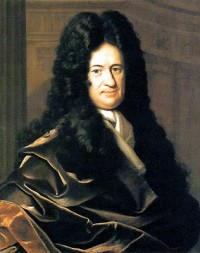
\includegraphics[height=0.2\textheight]{leibniz}
\end{center}

The German polymath Gottfried Wilhelm Leibniz occupies a grand place in the history of philosophy. He was, along with René Descartes and Baruch Spinoza, one of the three great 17th Century rationalists, and his work anticipated modern logic and analytic philosophy. Like many great thinkers before and after him, Leibniz was a child prodigy and a contributor in many different fields of endeavour.

But, between his work on philosophy and logic and his day job as a politician and representative of the royal house of Hanover, Leibniz still found time to work on mathematics. He was perhaps the first to explicitly employ the mathematical notion of a function to denote geometric concepts derived from a curve, and he developed a system of infinitesimal calculus, independently of his contemporary Sir Isaac Newton. He also revived the ancient method of solving equations using matrices, invented a practical calculating machine and pioneered the use of the binary system.

Like Newton, Leibniz was a member of the Royal Society in London, and was almost certainly aware of Newton’s work on calculus. During the 1670s (slightly later than Newton’s early work), Leibniz developed a very similar theory of calculus, apparently completely independently. Within the short period of about two months he had developed a complete theory of differential calculus and integral calculus (see the section on Newton for a brief description and explanation of the development of calculus).

Unlike Newton, however, he was more than happy to publish his work, and so Europe first heard about calculus from Leibniz in 1684, and not from Newton (who published nothing on the subject until 1693). When the Royal Society was asked to adjudicate between the rival claims of the two men over the development of the theory of calculus, they gave credit for the first discovery to Newton, and credit for the first publication to Leibniz. However, the Royal Society, by then under the rather biassed presidency of Newton himself, later also accused Leibniz of plagiarism, a slur from which Leibniz never really recovered.

Ironically, it was Leibniz’s mathematics that eventually triumphed, and his notation and his way of writing calculus, not Newton’s more clumsy notation, is the one still used in mathematics today.

In addition to calculus, Leibniz re-discovered a method of arranging linear equations into an array, now called a matrix, which could then be manipulated to find a solution. A similar method had been pioneered by Chinese mathematicians almost two millennia earlier, but had long fallen into disuse. Leibniz paved the way for later work on matrices and linear algebra by Carl Friedrich Gauss. He also introduced notions of self-similarity and the principle of continuity which foreshadowed an area of mathematics which would come to be called topology.

\begin{flushright}
  From \url{http://www.storyofmathematics.com/17th_leibniz.html}.
\end{flushright}

\clearpage
\subsection*{Questions}
\begin{questions}
  \question Find the derivatives:
    \begin{parts}
      \part $ \od{y}{x} $ if $ y = \sin x \ln x $.
      \part $ \od{y}{x} $ if $ y = x \sec kx $ ($ k $ constant).
      \part $ \od{f}{\theta} $ if $ f(\theta) = \frac{\cos \pi \theta}{\sin \pi \theta + \cos \pi \theta} $.
      \part $ \od{y}{t} $ if $ y = \cos^4 (\sin^3 t) $.
    \end{parts}
  \question The force $ F $ acting on a body with mass $ m $ and velocity $ v $ is the rate
            of change of momentum, $ F = \od{}{t} [mv] $. If $ m $ is constant, this becomes $ F = ma $,
            where $ a = \od{v}{t} $ is the acceleration of the body. However, due to relativistic
            effects, the mass of a particle varies with $ v $ as
            \begin{displaymath}
              m = \frac{m_0}{\sqrt{1 - \dfrac{v^2}{c^2}}},
            \end{displaymath}
            where $ m_0 $ is the rest mass of the body and $ c $ is the speed of light. Show that
            \begin{displaymath}
              F = \frac{m_0 a}{\left(1 - \dfrac{v^2}{c^2}\right)^{\frac{3}{2}}}.
            \end{displaymath}
  \question Recall that if $ \theta $ is given in degrees, then $ \frac{\pi \theta}{180} $ is the equivalent angle in radians.
            Find the derivative of $ \sin \theta $ if $ \theta $ is given in degrees.
\end{questions}
\end{document}
